This section presents an overview of the survey results. The survey was sent to 60 developers, getting a response from 25\% of them, totaling 15 answers.

\section{Developers Profile}

The \ref{fig:reasons} image shows the percentage of developers who identify with the reasons to join and stay in Free and Open Source for Geospatial Community.

 Most of them report joining the community to share knowledge and skills, learn and develop new skills, participate in the FOSS scene, participate in a new form of cooperation and improve products of other developers. In the \ref{fig:year} we can see that the year of the first experience in FOSS is well distributed along the years, starting from 1992 and ending in 2020. This reflects the fact that it is a solid and very closed community.

\begin{figure}[]
     \centering
     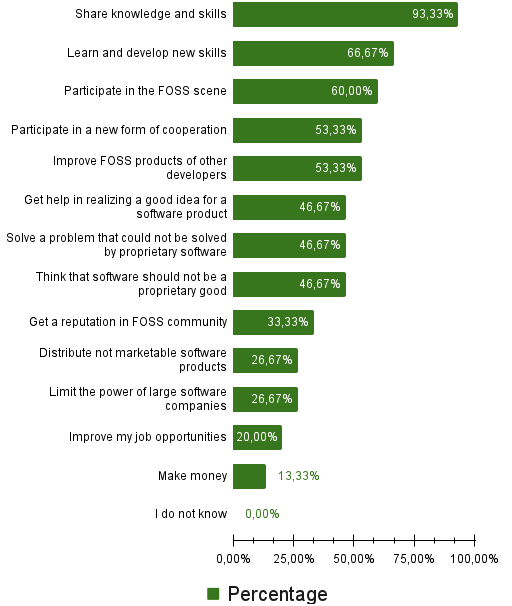
\includegraphics[scale=0.7]{img/reaons.png}
     \caption{Reasons to join and to stay in Free and Open Source Software (FOSS) for Geospatial Community}
     \label{fig:reasons}
\end{figure}
 
\begin{figure}[]
     \centering
     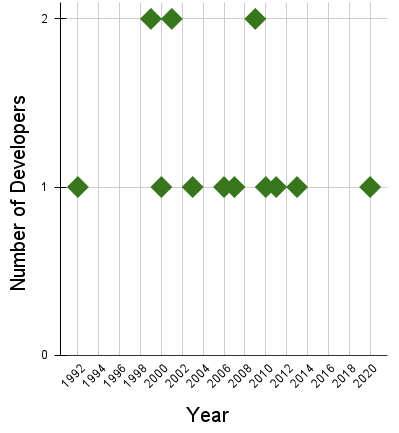
\includegraphics[scale=0.7]{img/year.png}
     \caption{Year of the first experience in Free and Open Source Software for Geospatial Community}
     \label{fig:year}
\end{figure}


\begin{figure}[]
     \centering
     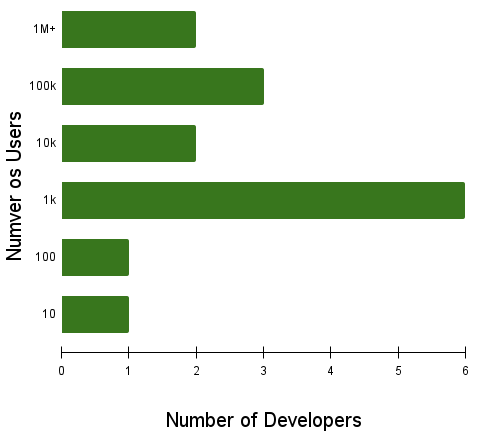
\includegraphics[scale=0.8]{img/users.png}
     \caption{ Number of users in the biggest project you are involved}
     \label{fig:users}
\end{figure}
In the figure \ref{fig:users} it is possible to observe that most of the developers are involved in big projects, and the responding developers who have projects with more than 100,000 users started in the FOSS community until 2003.

One of the biggest concerns when choosing respondents for the survey was choosing experienced users in the implementation of at least one of the proposed approaches. The results of the figure \ref{fig:apixp} show that 80\% of the respondents have some familiarity with the implementation or use of an API based on some specification of the OGC API. 

For the legacy service (figure \ref{fig:wsxp}), OGC Web Service, more than 93\% of respondents were familiar with it, with 86.7\% being developers who have already implemented a Web Service client or server. 

\begin{figure}[H]
     \centering
     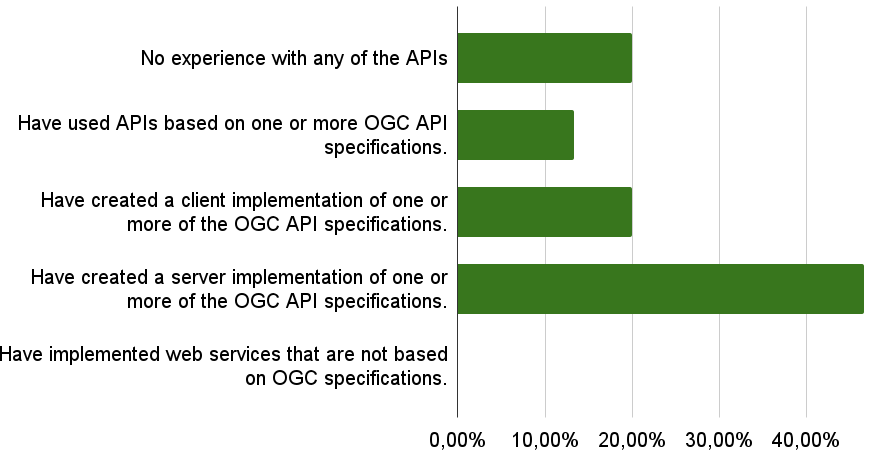
\includegraphics[scale=0.5]{img/apixp.png}
     \caption{Experience with the OGC API specifications }
     \label{fig:apixp}
\end{figure}

\begin{figure}[H]
     \centering
     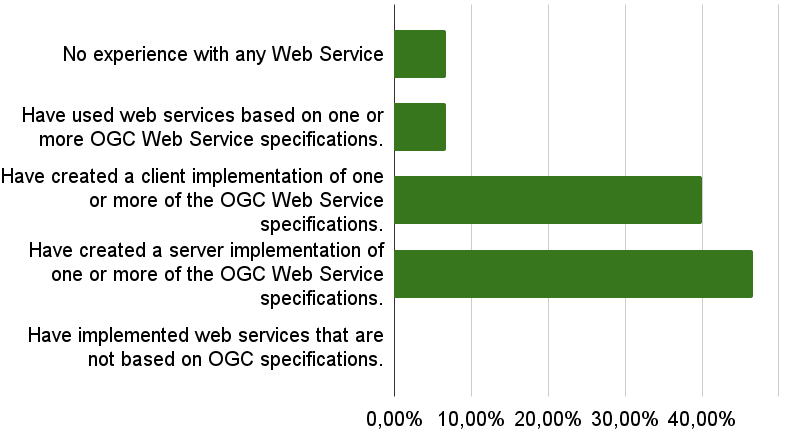
\includegraphics[scale=0.55]{img/wsxp.png}
     \caption{Experience with the OGC Web Service specifications }
     \label{fig:wsxp}
\end{figure}

The results of this section show the maturity of the public selected to respond to the survey. This guarantees less bias from users who are not familiar with the OGC API or OGC Web Services and are not well-educated on what is the OGC API.

\section{Software Evaluation}

For effort evaluation (figure \ref{fig:effort}) 66.63\% of participants answered "strongly agree" and "agree" that OGC API requires less resource and time to develop. Only one participant, with experience in creating a server implementation of both API and Web Service, disagreed with this statement.

\begin{figure}[H]
     \centering
     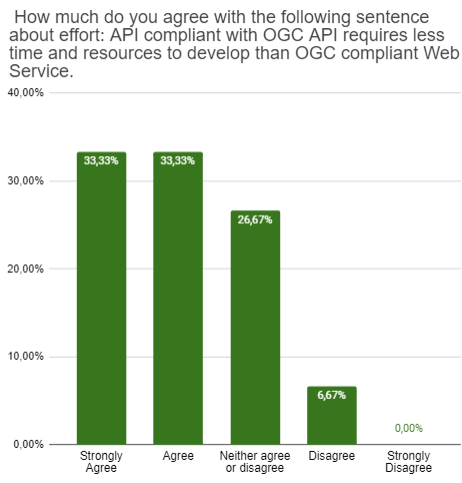
\includegraphics[scale=0.9]{img/effort.png}
     \caption{Effort Comparison}
     \label{fig:effort}
\end{figure}


\begin{figure}[H]
     \centering
     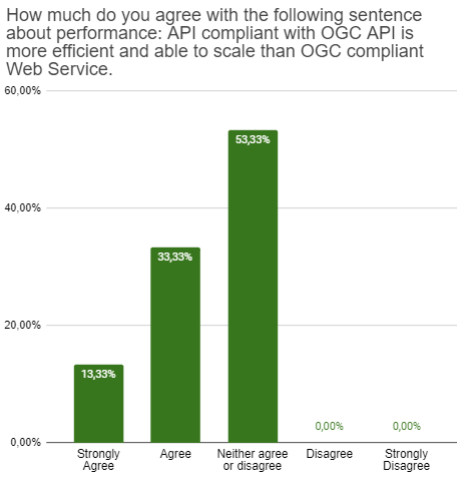
\includegraphics[scale=0.9]{img/performance.png}
     \caption{Performance Comparison}
     \label{fig:performance}
\end{figure}

\begin{figure}[H]
     \centering
     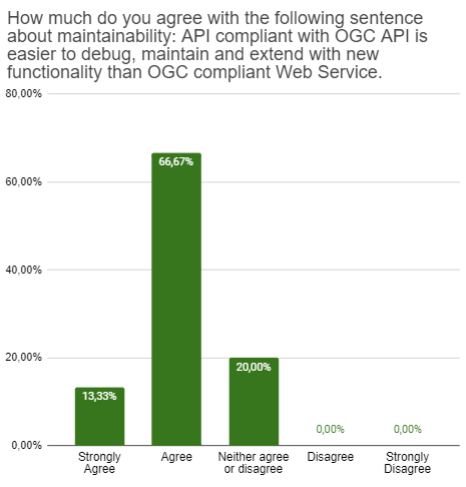
\includegraphics[scale=0.8]{img/maintain.png}
     \caption{Maintainability Comparison}
     \label{fig:maintain}
\end{figure}

Participants responses (figure \ref{fig:performance}) indicate that no developer believes that the Web Service performs better, but more than 50\% of the participants answered "neither agree or disagree". 46.6\% of participants believe that the API approach is more efficient and able to scale than OGC compliant Web Service.


\begin{figure}[H]
     \centering
     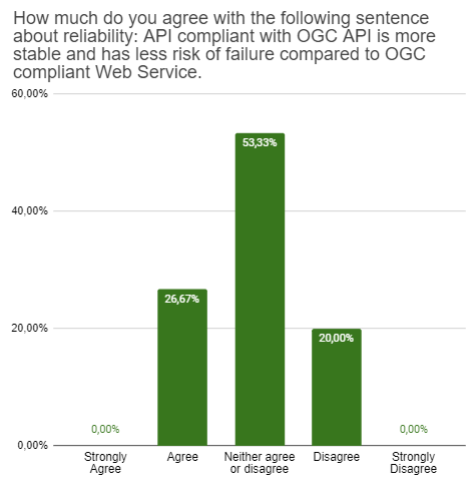
\includegraphics[scale=0.8]{img/reliability.png}
     \caption{Reliability Comparison}
     \label{fig:reliability}
\end{figure}

None of the participants believe that an OGC-compliant Web Service is easier to maintain than an API (figure \ref{fig:maintain}). 80\% of responses show that they believe API is easier to maintain, debug and extend functionality. Statement that maintains agreement with recent studies on the ease of implementing an API.


The developers demonstrated that there is no clear agreement on which approach has the highest reliability. Although the literature concludes that the REST approach is missing its own security model \cite{tihomirovs2016comparison}, the survey indicates that the tendency of participants is to believe that the API is more secure (figure \ref{fig:reliability}).


\section{Future of OGC API}


\begin{figure}[H]
     \centering
     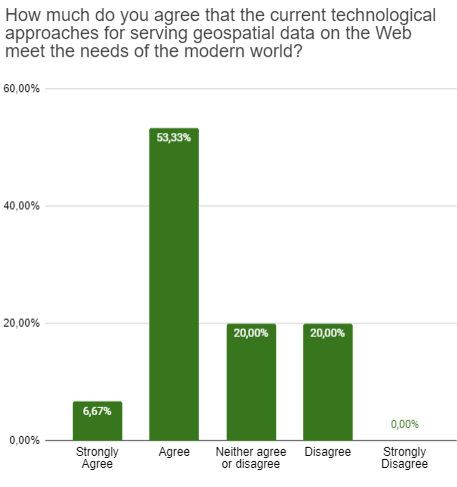
\includegraphics[scale=0.8]{img/modern.png}
     \caption{}
     \label{fig:modern}
\end{figure}

Most participants, around 60\%, believe that the current technological approaches for serving geospatial data on the Web meet the needs of the modern world, only 20\% disagree (figure \ref{fig:modern}).

The OGC API family has several standards for different types of spatial data and their metadata. From the 14 standards, five types were chosen that have not yet completed all the standards documents. Features is the most used standard, consequently it had the most applicable responses, the participants' opinion is distributed between minor, moderate and major gap. A major gap was also observed in the standard of Environmental Data Retrieval (EDR) and Records (a metadata standard). The 3D Volumes pattern got 70\% "not applicable" responses showing that developers are not yet widely using the standard.


\begin{figure}[H]
     \centering
     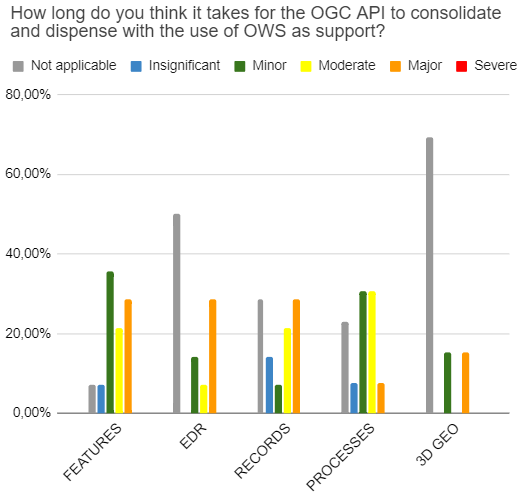
\includegraphics[scale=0.84]{img/gap.png}
     \caption{
     Functionality Gap between the standards families}
     \label{fig:gap}
\end{figure}



\begin{figure}[H]
     \centering
     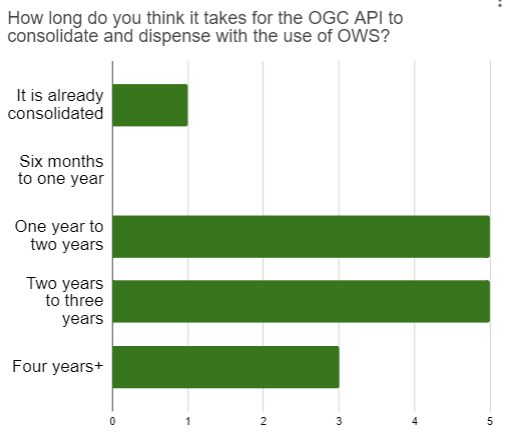
\includegraphics[scale=0.7]{img/consolidate.png}
     \caption{Time to OGC API to consolidate}
     \label{fig:consolidate}
\end{figure}

As can be seen in figure \ref{fig:consolidate}, only one person stated that the OGC API is already consolidated, no participant believes that the OGC API will be consolidated within a year. The other 92\% believe that it will be consolidated in at least one year.
